\subsection[Генераторы с нелинейными преобразованиями]{Генераторы с нелинейными \protect\\ преобразованиями}
\selectlanguage{russian}

Известно, что любая булева функция $f(x_1, x_2,  \dots, x_M)$ может быть единственным образом записана многочленом Жегалкина\index{многочлен!Жегалкина}:
\[ \begin{array}{ll}
    f(x_1, x_2, \dots, x_M) & = ~c~ + \\
    & + \sum\limits_{1 \leq i \leq M} c_i x_i + \\
    & + \sum\limits_{1 \leq i < j \leq M} c_{i,j} x_i x_j + \\
    & + \sum\limits_{1 \leq i < j < k \leq M} c_{i,j,k} x_i x_j x_k + \\
    & + \dots + \\
    & + ~ c_{1,2,\dots,M} ~ x_1 x_2 \dots x_M.
\end{array} \]

%Криптографу рекомендуется выбирать булеву функцию с возможно большим числом ненулевых коэффициентов при квадратичных членах полинома Жегалкина.

Второй способ улучшения криптостойкости последовательности поясняется с помощью рис.~\ref{fig:lfsr-zhegalkin}, на котором представлен регистр сдвига с $M$ ячейками и устройство, осуществляющее преобразование с помощью булевой функции $f(x_1, x_2, \dots, x_M)$, причем функция $f$ содержит нелинейные члены, то есть произведения $x_i x_j \dots$. Тактовый вход здесь такой же, как у регистров, показанных на других рисунках.

Если функция $f$ нелинейная, то в общем случае неизвестен полиномиальный алгоритм восстановления состояния регистров по нескольким последним выходам генератора. Таким образом, использование нескольких регистров сдвига увеличивает максимально возможный период по сравнению с одним регистром до $T < 2^{L_1 + L_2 + \dots + L_M}$, а нелинейность функции $f$ позволяет избежать простого нахождения состояния по выходу. Чтобы улучшить криптостойкость последовательности, порождаемой регистром, рекомендуется брать много нелинейных членов многочлена Жегалкина.

Такой подход применен в системе GPS. Удачных попыток ее взлома до сих пор нет.

\begin{figure}[!ht]
    \centering
	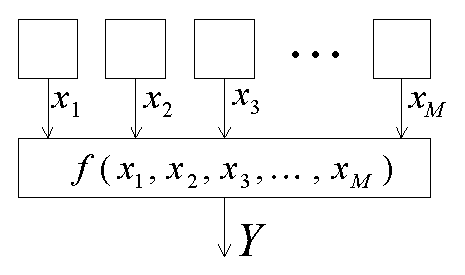
\includegraphics[width=0.4\textwidth]{pic/lfsr-zhegalkin}
    \caption{Криптографический генератор с нелинейной булевой функцией\label{fig:lfsr-zhegalkin}}
\end{figure}
